\documentclass[11pt,a4paper,twoside]{report}

% Aberstwyth dissertation LaTeX Template
% Authors: Dr. Hannah Dee (hmd1@aber.ac.uk), Neil Taylor (nst@aber.ac.uk)
% This has been adapted from the Leeds Thesis template and the 
% Group Project template for Computer Science in Aberystywth University.
% 
% All comments and suggestions welcome.
%
% Template designed to be used with pdflatex: it may need alteration to
% run with a different LaTeX engine

% To build document on the unix command line, run four commands:
 
% pdflatex dissertation
% bibtex dissertation
% pdflatex dissertation
% pdflatex dissertation

% you will end up with dissertation.pdf 
\usepackage{mmp}

% the following packages are used for citations - You only need to include one. 
%
% Use the cite package if you are using the numeric style (e.g. IEEEannot). 
% Use the natbib package if you are using the author-date style (e.g. authordate2annot). 
% Only use one of these and comment out the other one. 
%\usepackage{cite}
\usepackage{natbib}
\usepackage{graphicx}

\usepackage[official]{eurosym} % for the € (euro currency) symbol
\usepackage{paralist} % for inline lists
\usepackage{alltt} % for formating in verbatim environments.
\usepackage{listings} % for word wrapped code listings
\lstset{breaklines=true}

\usepackage{hyperref}
\hypersetup{
	pdfauthor={Steven Meyer \textless{}svm9@aber.ac.uk\textgreater},
	pdfsubject={CS39440: Major Project},
	pdftitle={Propel Designer},
	pdfkeywords={project, dissertation, propel, modelling, modeling, relation, entity, grammar, masters, bachelors, meng, aberystwyth, university, major, computer science, comp sci, er, rm, erd, xml, schema, schemas, schemata},
	pdfstartview={FitH}
}

% Use the following to selectively exclude chapters
%\includeonly{cover,abstract,acknowledge,declare,chapter1,chapter2}

\begin{document}

% all of the include directives below refer to tex files
% so 
\title{Propel Designer}

% Your name
\author{Steven James Meyer}

% Your email 
\authoremail{svm9@aber.ac.uk}

\degreeschemecode{G601} %e.g. G400 
\degreeschemetitle{Software Engineering} % e.g. Computer Science
\degreetype{MEng}

\modulecode{CS39440} % i.e. CS39440, CC39440, CS39620
\moduletitle{Major Project} % i.e. Major Project or Minor Project

\date{\today} % i.e. the date of this version of the report

\status{Release} % Use draft until you create the release version. Then, change this to Release.
\version{1.0}

%The title and name of your supervisor.
\supervisor{Prof.\ Reyer Zwiggelaar} 

%The email for your supervisor. 
\supervisoremail{rrz@aber.ac.uk}

\maketitle



 includes cover.tex - to change the content,
% edit the tex file

\pagenumbering{roman}

% This is the front page

\title{Propel Designer}

% Your name
\author{Steven James Meyer}

% Your email 
\authoremail{svm9@aber.ac.uk}

\degreeschemecode{G601} %e.g. G400 
\degreeschemetitle{Software Engineering} % e.g. Computer Science
\degreetype{MEng}

\modulecode{CS39440} % i.e. CS39440, CC39440, CS39620
\moduletitle{Major Project} % i.e. Major Project or Minor Project

\date{\today} % i.e. the date of this version of the report

\status{Release} % Use draft until you create the release version. Then, change this to Release.
\version{1.0}

%The title and name of your supervisor.
\supervisor{Prof.\ Reyer Zwiggelaar} 

%The email for your supervisor. 
\supervisoremail{rrz@aber.ac.uk}

\maketitle



                        

% Set up page numbering
\pagestyle{empty}

% declarations of originality
\clearpage
\hfill
\clearpage 
\thispagestyle{empty}

%%%
%%% You must sign the declaration of originality. 
%%%
\begin{center}
    {\LARGE\bf Declaration of originality}
\end{center}

In signing below, I confirm that:

\begin{itemize}
\item{This submission is my own work, except where clearly
indicated.  }

\item{I understand that there are severe penalties for plagiarism 
and other unfair practice, which can lead to loss of marks
or even the withholding of a degree. }
 
\item{I have read the sections on unfair practice in the Students' 
Examinations Handbook and the relevant sections of the 
current Student Handbook of the Department of Computer 
Science.}
 
\item{I understand and agree to abide by the University's
regulations governing these issues.}
\end{itemize}

\vspace{3em}
Signature ............................................................  \\

\vspace{1em}
Date ............................................................ \\

%%% 
%%% We would like to make a selection of final reports available to students that take 
%%% this module in future years. To enable us to do this, we require your consent. You 
%%% are not required that you do this, but if you do give your consent, then we will have 
%%% the option to select yours as one of a number of reports as examples for other 
%%% students. If you would like to give your consent, then please include the following 
%%% text and sign below. If you do not wish to give your consent, please remove this 
%%% from your report. 
%%%
\vspace{5em}
\begin{center}
    {\LARGE\bf Consent to share this work}
\end{center}

In signing below, I hereby agree to this dissertation being made available to other
students and academic staff of the Aberystwyth Computer Science Department.  

\vspace{3em}
Signature ............................................................  \\

\vspace{1em}
Date ............................................................ \\

               

\thispagestyle{empty}

\begin{center}
    {\LARGE\bf Acknowledgements}
\end{center}

I'd like to thank...
\begin{itemize}
	\item My supervisor, Professor Reyer Zwiggelaar, for allowing me to create this project at my own pace and for encouraging me to do my best.
	\item My long-suffering partner, Aylin Alieva, for putting up with me throughout all of my years at the University, but particularly for these final months of dissertation work. 
	\item The Father and the Son, for giving me strength.
\end{itemize}
 % Acknowledgements
\thispagestyle{empty}

\begin{center}
    {\LARGE\bf Abstract}
\end{center}
% 210 words

Databases can be usefully modelled as Entity Relationship Diagrams (ERDs). Such diagrams use visuals to show information about database schemata such as relationships and cardinalities, entities and attributes in a way which is easy for a human to recognise. Colouring and emphasis can further assist in using ERDs as a useful tool for sharing and communicating a database schema.
\\

Propel is an open-source Object-Relational Mapping (ORM) for PHP. It creates objects to allow for programmatic database manipulation and for database abstraction. It creates these objects and the database implementation from schema files. These schemata define the tables, columns, keys, indices and relations and their attributes within a database.
\\

Schema files are coded in XML. While this makes them understandable so far as the data is marked-up in a human-readable manner, it makes sharing and collaborating difficult. The linear structure makes it difficult to see the structure and relationships. This, in turn, makes it difficult to ensure that the schema is modelling the domain and following business logic correctly. They are also not very friendly for the less technically-inclined.
\\

It can be seen, then, that it would be useful to have a tool which can be used to manipulate Propel schemata by means of direct XML manipulation and by ERDs.                 % Abstract 210 words

\pagenumbering{roman}
\pagestyle{fancy}
\fancyhead{}
\fancyfoot[C]{\thepage}
\renewcommand{\headrulewidth}{0 pt}
\renewcommand{\chaptermark}[1]{\markboth{#1}{}}

\tableofcontents   
\newpage
%\listoffigures
%\newpage 
%\listoftables
%\newpage
\clearpage
\hfill
\clearpage

% Set up page numbering
\pagenumbering{arabic}

\setchapterheaderfooter

% include the chapters
\cleardoublepage
\chapter{Background \& Objectives} % 976 words
\section{Background}
Data modelling and database design are vast topic areas accompanied by many volumes of published theory and literature. This project focusses on a fragment of the topic; conceptual design\slash schemata. Specifically, it is concerned with entity relationship (ER) grammar and mainly with ER diagrams.

The ER modelling grammar for conceptual modelling serves two major purposes. Firstly, it can be used as a communication device used by an analyst to interact with an end-user. Secondly, it can be used as a design tool at the highest level of abstraction to communicate a deeper understanding to the database designer (\cite{DataModelingAndDatabaseDesign}). Id est the database structure and semantics can be described in a manner which is not specific to any implementation.

Where object relational mapping (ORM) is used, such diagrams can also be useful devices for describing the relationships between objects to the application programmers. This is particularly useful where business logic is applied at the application level; developers (who may not have designed the database, themselves) must have a way to understand the logic represented by the database design and to understand those parts of the business logic which must be applied at the application level. This is particularly relevant when using an ORM such as Propel, where the level of database abstraction afforded to the application programmers comes at the price of losing the ability to describe logic at the database level. Database-level logic, in this case, is represented by stored procedures, triggers et cetera.

For the ORM Propel, database schemata are described as XML files. These descriptions are a mixture of database instruction such as entities (tables), attributes (columns) and simple referential actions for deletion and updating of rows, and of PHP instructions for the generated PHP code.

These files make for more difficult traversal for application programmers and database engineering alike, as references must be searched for among the (possibly) many entity descriptions and indices are separately described from the attributes they reference. It is also far too tempting for application programmers to make changes to the schemata when requirements change. Maintaining any ER diagrams in such situations is a maintenance issue, and checking that the resultant schemata still correctly and properly represent the business logic becomes very difficult.

There exists many database modelling tools which support the creation and editing of ERDs. Many of these tools are useful tools for inspecting existing databases, providing support for many different back-ends. However, they are primarily aimed at SQL interaction with these databases, rather than at maintaining ER diagrams.

There are products which will natively support ER diagrams and ORM frameworks, but these products are not free software. Existing software, as it stands, usually has one of these weaknesses:
\begin{itemize}
	\item They do not support ORM. They support different databases, but cannot be made to work with an ORM schema.
	\item They do not support ERDs or relational modelling schema (a form of physical data modelling).
	\item They are not free software. They are either not \emph{gratis} (without cost) or not \emph{libre} (without restrictions) or both.
\end{itemize}

This project, rather than being of commercial importance or even being a common problem in industry, came about by the student's own need. Such a situation, however, is the precursor to every good work of software (\cite{CatB}).

\section{Objectives}
The most basic aim of this project is to build a free tool to create ER\slash RM diagrams from Propel schema XML and vice versa. It should provide the expected features of existing modelling tools, but be specifically aimed at Propel schemata. The normalised information-preserving grammar of Propel is more closely related to relational modelling grammar, so RM modelling grammar would be preferable to ER modelling grammar.

The core goals of the project are:
\begin{itemize}
	\item To produce an schema diagram consisting of
	\begin{inparaenum}[(\itshape i\upshape)]
		\item tables,
		\item relationships
		\item attributes (and their types) and
		\item cardinality notations
	\end{inparaenum}
	using a Propel schema as input.
	\item To make such a diagram interactive\slash editable with a database modelling tool.
	\item To produce a Propel schema XML using a schema diagram as input, id est the reverse of goal 1.
	\item To be gratis to use.
\end{itemize}

The project had these stretch goals which were available if the core goals were to be achieved in good time:
\begin{itemize}
	\item Further integration with Propel to allow for additional logic such as validators and behaviours.
	\item Include inheritance. This is part of the Propel schema and introduces aspects of enhanced ER modelling.
	\item To be portable. These tasks do not require any OS interaction and so should not need installing, neither should any special software be required to use it.
	\item To make use of only free and open standards. The software should not include any closed-source technology.
	\item To be free software, id est libre.
\end{itemize}

\section{Related Systems}
As previously discussed, there are many existing `database designers' available. One such product which has native support for ORMs, including Propel, is ORM Designer. However, this product is closed-source and costs \euro99 for a single licence.

The initial design for this project was to extend an existing software to include support for Propel schema. Of the various free modelling tools which were investigated, WWW SQL Designer by Ond\v{r}ej \v{Z}\'{a}ra was selected to be extended. This designer produces its own XML from RM diagrams, and database-specific SQL is generated from this using XSL transforms. The software is written in JavaScript and HTML meaning that it should run on any platform with a web browser making it a portable application and fulfilling one of the goals of this project.

There are flaws in the software, however, which limited its usefulness for modelling Propel schema (or, indeed, any database) such as lack of composite key support and other incompatibilities with transforming the XML. It also used an in-house JavaScript library created by Zara which made modifying the code to add extra features a challenge. It also has no facility to save the diagram as an image.

After these issues were identified, it was decided that the modelling software would be created as part of this project to utilise modern web technology and avoid custom frameworks.% 1178 words
%\addcontentsline{toc}{chapter}{Development Process}
\cleardoublepage
\chapter{Development Process}% 942 words

%You need to describe briefly the life cycle model that you used. Do not force your project into the waterfall model if it is better described by prototyping or some other evolutionary model. You do not need to write about all of the different process models that you are aware of. Focus on the process model that you have used. It is possible that you needed to adapt an existing process model to suit your project; clearly identify what you used and how you adapted it for your needs.

%In most cases, the agreed objectives or requirements will be the result of a compromise between what would ideally have been produced and what was felt to be possible in the time available. A discussion of the process of arriving at the final list is usually appropriate.

%You should briefly describe the design method you used and any support tools that you used. You should discuss your choice of implementation tools - programming language, compilers, database management system, program development environment, etc.

%\section{Introduction}
%Introduce the specific model that you chose to use. 

%\section{Modifications}
%Did you have to modify the model to suit a one-person project. If so, what did you change and why? 

% STILL NEED TO TALK ABOUT RELEASE PLANNING AND ITERATION PLANNING
\section{Process Methodology}
\subsection*{Selection}
A schema diagram consists of a few main parts: the tables; the columns; and relationships. These are hierarchical in nature --- tables have columns, columns have attributes and relationships depend on tables most significantly and then on columns. When viewed in this manner, it can be seen that an evolutionary process model can be used to develop the system.

It was decided than an agile approach to development would be used. The developer was also the intended customer for this project, although the software would presumably be usable by others, so the developer team would be small and the customer dedicated, collaborative, and empowered. As the system is evolutionary in nature, the requirements can be detailed as and when they are required, rather than being described in their entirety from early in the project.

The development process was mostly based upon elements of extreme programming (XP), adopting those facets pertaining to fast, iterative programming such as ``you ain't gonna need it'' (YAGNI) and test-driven development (TDD). The requirements and tasks were formed using XP's notion of stories.

In using this development model, it should have been the case that after every iteration there would be a functional (if not feature-laden) product. This gave some protection against unforeseen changes or set-backs, assuring that there would be a product at every stage of the life-cycle. It would also deliver value early in the production.

Once the development methodology had been chosen the high-level requirements stories were described. These initial stories were very simplistic in their specification and encapsulated the main aspects of forming a diagram of an entity. Due to the use of XP, failure to implement any of these stories would not affect the releasable state of the program.

When the original modelling tool was abandoned, these same high-level stories were re-usable in specifying the development of the new modelling tool after having their context altered to fit.

\subsection*{Modification}
Some XP components had to be modified to cater to the requirements of the project. As the project was being undertaken by a sole developer, the practice of pair programming could not be accomplished in the expected way. As pair programming is an essential device for detecting and correcting errors and code smells, it was adapted to have some impact with a sole developer: the code was inspected at a later date in order to identify issues which had been missed in the first instance.

The YAGNI process was also relaxed slightly in order to accommodate for patterns for which it was clear would be required at a later date, but which would be prohibited by an XP purist as such action would be deemed superfluous in the instance in which it was being created. This decision was intended to reduce the amount (and cost) of refactoring which would be required when the XP process would eventually call for it.

\subsection*{Requirements Specification}
Stories were committed to story cards to be arranged on a board in the vicinity of the development environment, but for stories which had been broken down into detailed tasks were committed to tickets using Trac. This program allows for tickets to be assigned, have comments added, and ultimately closed as completed allowing the work-flow to be documented and visualised.

\section{Tools}
The first implementation of the software was written in XSLT and JavaScript --- the same programming languages as the intended design tool, \mbox{WWW SQL Designer}. The final implementation which included a designer used JavaScript, scalar vector graphics (SVG), and HTML5. These programming languages were selected because of their ubiquitous support on all major platforms; all of these are available in most major web browsers. It was decided that the Java\-Script would be compiled from Coffee\-Script. This is mainly due to Coffee\-Script's standardised way of dealing with classes in Java\-Script and because the compiled Java\-Script is purportedly more readable than and executes as fast as or faster than equivalent JS written without Coffee\-Script and which is also pretty-printed and passes through JSLint without generating warnings (or errors).

The tests for the TDD process where created using unit testing frameworks for the programming language being used. For the initial development iteration being integrated with WWW SQL Designer, the XSLT style-sheets were tested by creating unit tests to be used with XSLTunit. This framework used XSLT documents as tests applied on the XSLT document to be tested in order to produce results as XML. The transformations are initiated by a web page using Java\-Script, but the tests could be carried using any engine which can apply XSL transforms.

The Coffee\-Script was tested using JsUnit, running the tests on the Java\-Script produced by compiling the Coffee\-Script into Java\-Script. JsUnit tests are composed in Java\-Script and the tests are run and aggregated by an HTML web page which displays the results and gives details of the errors.

Continuous Integration suites were not used due to the size of the project and the effort required to integrate a CI suite. The benefits which using such a suite would have brought to the project were emulated to some extent by running the suite of tests whenever the code-base was altered and when new tests were created. This ensured that modifications and new code did not affect the working state of other code in the project.

All development was performed using the Netbeans IDE from Oracle Corp. The release candidate version 7.3 was selected for its enhanced HTML5 development environment and the Coffee\-Script plug-in was used for developing and compiling Coffee\-Script. Using this IDE allowed the project to be debugged in the IDE, negating the need for additional web-browser inspection tools.% 1321 words
\cleardoublepage
\chapter{Design}% 2647 words



%You should concentrate on the more important aspects of the design. It is essential that an overview is presented before going into detail. As well as describing the design adopted it must also explain what other designs were considered and why they were rejected.

%The design should describe what you expected to do, and might also explain areas that you had to revise after some investigation.

%Typically, for an object-oriented design, the discussion will focus on the choice of objects and classes and the allocation of methods to classes. The use made of reusable components should be described and their source referenced. Particularly important decisions concerning data structures usually affect the architecture of a system and so should be described here.

%How much material you include on detailed design and implementation will depend very much on the nature of the project. It should not be padded out. Think about the significant aspects of your system. For example, describe the design of the user interface if it is a critical aspect of your system, or provide detail about methods and data structures that are not trivial. Do not spend time on long lists of trivial items and repetitive descriptions. If in doubt about what is appropriate, speak to your supervisor.


\section{Overall Architecture}%Emergent design
The system was to be produced using agile\slash XP principles, so  it should have been the case that the ideas of emergent design would give rise to a coherent design and good software as the project developed. Even with this principle in effect, it was clear that there was an overall design inherent to the project which separated it into distinct parts. These parts are:
\begin{itemize}
	\item The database model.
	\item The diagram modelling tool and its interface.
	\item Code to link the previous two parts and to also transform the model into XML.
\end{itemize}

With these parts, it could be seen that the design pattern model-view-controller (MVC) would be a suitable pattern for the overall design.

As the entire software was to be run on a single machine, all of the programming was designed with Java\-Script and its merits and limitations in mind.

\section{Stories}
The model, view and controller parts were not created as separate entities in isolation, as may be the case with a plan-driven process, but they evolved together over time as stories were implemented.

A story would describe a design so broad as ``As a user, I need to add tables to a database so that my database has entities.'' This would then be separated into its tasks for the model and for the view. These would be tasks such as ``A database should maintain a collection of tables'' and ``A database should allow tables to be added to its collection'', which would both be tasks for the model. The related tasks for the view would be similar; ``It should be possible to add a table to the database''.

Following the principles of test-driven development, these tasks were used to create a black-box style test. Id est an expected outcome would be described and the test was considered satisfied provided that it passes, regardless of how the code accomplished the task. For example, a test would expect the outcome that the SVG has a new \emph{rect} (rectangle) element of the class `rect' after adding a table; how that came to be was not significant.

\section{Coding Style}\label{sec:CodingStandards}
\subsection{OOP and JavaScript}
The model was designed to be entirely object-oriented. Java\-Script is not a class-based language as Java is and, unlike most OO languages, has a variety of patterns for supporting OO programming styles.

CoffeeScript provides a class structure in order to simplify attaching functions to the prototype chain and also correctly handles the setting of the superclass. Coffee\-Script uses the pseudo-classical pattern. In this pattern, objects are created with the \texttt{new} keyword and a constructor function --- similar to conventional OO languages --- and (public) methods are attached to the object prototype.

The prototype is used when member isn't found on the object itself. For example, if the object \texttt{foo} has no member \texttt{foo.bar}, then the engine looks for the object's constructor's prototype. This prototype object is inherited and, when used in this way, conserves memory as the members do not need to be copied to each instance.

Prototype members are \emph{live} members; changes to the prototype will affect all current and future instances of the object. As a result, it is not a useful pattern for private members. The conventional handling of private members for this pattern is to prepend their names with an underscore. While this is useful for creating `protected' members (Java\-Script has no support for true protected members), it still exposes the member publicly as both readable and writeable.

In order to handle private members, it was decided that the all-in-one constructor pattern would also be used, but only for this purpose. This pattern adds all members to the object in the constructor and doesn't make use of the prototype at all. This is not entirely desirable, as inheritance breaks down somewhat (the \texttt{instanceof} keyword doesn't work, here) and every instance carries all of its members (no shared prototype object). It does encapsulate private members, though, and the pattern allows for the creation of `privileged' members; publicly accessible members which have access to private members.

It was decided that all Java\-Script objects would follow these rules:
\begin{itemize}
	\item Private members would be defined in the constructor (all-in-one constructor pattern).
	\item Public members requiring access to private members (privileged members) would be defined in the constructor (all-in-one constructor pattern).
	\item Public members which are not privileged would be attached to the prototype (classical pattern).
\end{itemize}

\subsection{CoffeeScript}
Functions in Coffee\-Script are defined by the means of
\begin{alltt}variable = (param1, param2, \ldots, param\slshape{n}\upshape) -> function here\end{alltt}
Where a function has no specified parameters, it is permitted in Coffee\-Script to omit the brackets and start the function with the arrow (\texttt{->}). However, it was decided that functions without specified parameters would always include the empty brackets in order to clarify that the function is intended to have no parameters. It also serves an \ae{}sthetic function, causing it to become easier to identify functions.

Those variables in Coffee\-Script which hold jQuery objects are prefixed with the \$ symbol to differentiate them from references to non-jQuery variables. This was introduced part-way through the project when it became necessary to easily separate variables which reference jQuery objects. Because of this, there may be some earlier code which does not exhibit this coding style.

Functions, methods and variables were always to be defined in alphabetical order to make them easier to locate. This style could be contravened where the ordering was dictated by the code.

\section{Model}\label{sec:DesignModel}
\subsection{Structure}
The model was designed to closely model the Propel schema reference. The structure of the XML schema document was to be represented in the model. As and when the agile method required them, this lead to the creation of 6 objects: Database, Table, Column, Foreign Key, Index and Unique Index. Foreign Key, Index and Unique Index were consigned to iterations beyond the time-frame available to the project as modelling tables and columns were deemed to deliver the greatest value.

The schema hierarchy has columns contained within tables, which, in turn, are contained within a database element. This becomes problematic when one considers that each element can inherit attributes from its container. As tables are referenced from the database in the model (Database ``has a'' Table), the table would require a reference to the database object for its values. This approach would have introduced tight coupling into the software which was rejected as bad practice. In order to flag those values which were to be inherited to differentiate them from those with their own values, a static-like variable was introduced to the models. Values which were to be inherited from the container were set thus:
\begin{alltt}table.setPhpNamingMethod Table.INHERIT\end{alltt}
As the output XML would not require the true value, the inheritance would not need to be resolved by the software.

\subsection{Visibility}
As discussed in the previous section (\ref{sec:CodingStandards}), Java\-Script objects were created using a mix of the pseudo-classical and the all-in-one constructor patterns. This decision was particularly relevant to the objects in the model, as their attributes could either be public or private. Choosing one of these visibilities would change the pattern required for their access.

It was decided that attributes and collections would be private instance variables accessed by means of public get and set functions. This decision was made in the name of good practice. By mandating the use of these functions, any changes to the way in which attributes are get or set internally of the object would not require a change in the code which tries to get or set these attributes. As these functions are privileged, they follow the all-in-one constructor pattern.

By having the attributes and collections as publicly accessible properties of the objects, the code would have been easier to read and shorter, but it was rejected for the reasons already given and also for the reason that it would expose the internal data types, which are also liable to change.

\subsection{Programming Language}
JavaScript was selected as the programming language of choice by the merit of its inclusion on most platforms, devices and web browsers. Such penetration could not be matched by any other language available; Java requires a JVM installed and native programs are inherently restricted to their native platform. It also ties in conveniently with the other technology in use for the view and controller --- that of HTML5 and SVG. All three are available together in most modern web browsers.

\section{View}
While researching other database modelling software, it was discovered that an oft lacking feature in demand in the forums was the ability to save the diagram as an image. With this in mind, the decision was made to have the diagram as an image, rather than using some other display technology such as HTML\slash HTML5 canvas or Adobe Flash. By using an image as the view, it would remove the need to convert the model into an image at a later stage and all of the complexities and potential incompatibilities which would accompany such a choice. That which was visible in the view would be exactly that which was in any exported image.

\subsection{SVG}
Scalar vector graphics (SVG) are images created by XML. This means that they can be created and interacted with programmatically by means of manipulation of the SVG's DOM. Being a vector image format also gives any exported image can be scaled without any loss of quality, unlike rasterised bitmap images which are limited in their resolution.

SVG are supported by all major browsers in their modern versions. This has the implication that no extra software or plug-ins are required to use the software, unlike other rich technology such as Flash or Micro\-soft Silver\-light.

As the file is of an XML format, the semantics of the diagram and interface can be marked-up with ARIA attributes to improve the accessibility. This is unlike other RIA programs which may not have the same accessibility support as a web browser does.

SVG suffers from rendering speed degradation as DOM complexity increases. As this project will likely only be drawing a limited quantity of rectangles, text and lines per table, was deemed unlikely that this would cause problems for anything but very large schemata.

It was decided that jQuery would be used to interact with the SVG. Some of the jQuery library's function do not support SVG as completely as they do HTML, but these are clearly noted in the jQuery documentation and the work-arounds, where required, should not require a great deal of Java\-Script.

\subsection{HTML5 Canvas and HTML}
HTML5 canvas was considered due its Java\-Script API and its standalone support in major browsers. However, it was quickly rejected as it lacks the capability for dynamic components. In SVG the individual entities can be interacted with whereas the entire HTML5 canvas must be redrawn in order to alter it. Such behaviour would degrade the user experience for schemata with more than a few tables, as larger and larger canvasses (images) would need to be redrawn every time something is added, removed or moved as the number of tables increases.

HTML was considered for its superior support and superior accessibility, but the advantages of SVG caused HTML to be rejected. HTML would also require an interpreter to create an image of the diagrams.

\section{Controller and User Interface}
The controller was designed to maintain the Java\-Script model, ensure the integrity of the SVG view, and to handle the interaction between the two.

The controller was designed to be in two main parts: a jQuery plugin to interact with the view and an HTML5\slash Twitter Bootstrap API to allow the user to change the model and view. The latter consists of an HTML5 interface from which the user can add tables and such with some Java\-Script to control the model; the interface delegates view interaction to the jQuery plugin.

In order that this interface be testable, the components of the Twitter Bootstrap framework were created as Java\-Script objects which extend the jQuery object. Having the components as controllable objects instead of simple HTML to be inserted into the DOM allowed the interface to be constructed in such a way that it was predictable, testable and much simpler to read in the code. Rather than constructing many snippets of HTML, one can create an object and expect certain functions to be present. These functions replace the many jQuery functions required to do the same task with one function call. Having them extend jQuery enables them to function as jQuery object, with all of the functionality that jQuery allows.

Using the Twitter Bootstrap framework also presents the user with a familiar interface as the same framework is becoming more popular on the world wide web. It is also well tested and polished, reducing the work required for the user interface in this project.

Another key reason for using jQuery and Twitter Bootstrap is in the fact that both are designed to work well and consistently in all browsers and on all devices. This is important as it reduces the amount of work which would otherwise be required to work around the major and minor nuances of the different Java\-Script engines, rendering engines and platforms, such as the notoriously unwieldy Internet Explorer 7.

\section{Other Technology}
\subsection{Adobe Flash}
Adobe Flash has a scripting API available and is capable of performing as a user interface for the software. It is not a native part of a web browser or system, but is often present on many systems due to its pervasive usage for both local content and on the world wide web. However, Flash is in decline on mobile devices and Adobe has discontinued its support for mobile platforms. While this was not a reason to reject it (this project is not aimed at mobile support, yet), it sets a precedent for Flash's future as developers will not be too happy to produce desktop content in Flash and mobile content in HTML5.

Flash is also not an open standard and this fact combined with the previous information and the fact that taking the time to learn Flash would not have been in the best interests of the project resulted in Flash not being considered for use.
\subsection{Microsoft Silverlight}
Microsoft Silverlight is an application framework for RIAs. While this project does not require an internet connection, Silverlight could still have been used to create the project. The interfaces of Silverlight applications have an API accessible by a subset of Microsoft's .NET framework.

Silverlight is available on Linux and FreeBSD by the use of the Moonlight project. However, the team responsible for the project --- the Mono team --- have abandoned its development. There are also issues with the licensing agreement between Microsoft and Novell and the product's penetration and use (or lack thereof).

Silverlight was rejected for similar reasons to that of Flash.

\subsection{Java and JavaFX}
Oracle has recently introduced JavaFX for creating user interfaces using Java for Java applications and RIAs. JavaFX would not have been an unreasonable choice for developing the model and the view as it could support all of the features required for the model, view and controller and handled the interactions between them. Java was rejected in favour of Java\-Script, HTML5 and SVG as these are available without the need to install extra software on most platforms.

\section{Other design decisions}
\subsection{Boilerplate}
It was decided that the HTML5 boilerplate template generator \emph{Initializr} would be used to generate the base code to start the view and controller. This generator creates the index.html page which includes some boilerplate code for displaying correct content in browsers and it also includes the Twitter Bootstrap CSS and Java\-Script, the latest jQuery Java\-Script, the Modernizr feature detection Java\-Script and some extraneous pieces which are more useful for content which is to be served over the web.

Modernizr detects the HTML5 and CSS3 features which the browser supports. Initially, this is of limited use, but as the project progresses it may become useful to have feature detection. While this may seem at odds with the principles of agile development, Modernizr also includes scripts to add HTML5 functionality to browsers which don't support them natively and has been included for this reason.

%\section{Some detailed design}

%\subsection{Even more detail}

%\section{User Interface}

%\section{Other relevant sections}% 2647 words
\cleardoublepage
\chapter{Implementation} % 1750 words

%The implementation should look at any issues you encountered as you tried to implement your design. During the work, you might have found that elements of your design were unnecessary or overly complex, perhaps third party libraries were available that simplified some of the functions that you intended to implement. If things were easier in some areas, then how did you adapt your project to take account of your findings?

%It is more likely that things were more complex than you first thought. In particular, were there any problems or difficulties that you found during implementation that you had to address? Did such problems simply delay you or were they more significant? Your implementation might well be described in the same chapter as Problems (see below).

\section{WWW SQL Designer}
\subsection{XSLT}
The test-driven development of the XSLT for the initial version of the software was reasonably straight-forward. The main issues arose from the lack of familiarity with XSL transforms, generally, as instruction for executing certain transforms frequently had to be looked-up in the early stages of the development.

One drawback with using the XSLTunit framework was in the engine's lack of support for importing tree fragments from external documents. This issue stemmed from the engine's poor implementation of the EXSLT (XSLT extension) for importing tree fragments, rather than an issue with the unit testing framework. In not having this extension available, it became the case that XML had to be embedded in every test which was specific to that test in which it was embedded. Having one block of test XML would have ensured consistent behaviour from the XSLT, rather than the emergent situation where the tests only proved their validity with the XML in isolation. It also increased the size of the tests.

The XSL, alone, could not model the Propel schema in its entirety. The WWW SQL Designer software was intended to be a generic schema designer for as many different database back-ends as possible. In this regard, it has the same aims as Propel which aims to provide a level of abstraction from the database back-ends. However, the Propel schema adds Propel-specific instructions\slash attributes to the elements it describes, some of which do not have bearing on the databases, but should be included in the schema nonetheless.

\subsection{oz.js Library}
In order to extend the software to include this extra detail, the Java\-Script and user interface needed to be altered.

The original author of the software, Ond\v{r}ej \v{Z}\'{a}ra, has included a Java\-Script library of his own creation, oz.js, to handle advanced Java\-Script constructs such as custom events and class-like inheritance. This library is used extensively throughout the project. However, when examining the code in order to interact with the models, it was not possible to discover a method for extracting the models from the data structures in this library. Handles to the model object could be retrieved, but they were lacking the functions which seemed to be available inside of the library. This resulted in the models being uneditable without modifications to the library, which it was decided was outside of the scope of the project and would have required much learning in order to understand the library.

A post on the Google Code mini-site for the project suggested that the WWW SQL Designer project make use of the jQuery library, as this library has a larger user base and is better documented. This would allow developers to contribute to the project without requiring them to first learn how to use the new library.

It was this difficulty and the previously discussed post which prompted the decision to abandon the WWW SQL Designer project and create a new system from the ground up using more popular frameworks and libraries. The move would allow the designer to be built with Propel in mind and to address other issues with \v{Z}\'{a}ra's project, such as the ability to save the schema as an image.

\section{Propel Designer}\label{sec:PropelDesigner}
\subsection{CoffeeScript}
CoffeeScript was a new programming language for the developer and, as a result, had to be learnt in order that it would be usable. However, as the body of the code is either Java\-Script or code which compiles 1:1 into Java\-Script, the learning curve is minimised greatly. There were occasions where the language was so different that the code had to be prototyped in the Coffee\-Script real-time compiler on the Coffee\-Script website in order to discover exactly how to structure the required Java\-Script code as Coffee\-Script.

Coffee\-Script includes mechanisms to simplify OO programming and inheritance in Java\-Script. The ability to set out a `class' in Coffee\-Script in a similar way as one would in a language such as Java was very useful, as traditional OO languages such as Java were much better understood.

Classical OOP in Java\-Script is somewhat convoluted and its complexity often leaves it shunned for simpler patterns such as the prototypical Module pattern using functions and closures. Indeed, many libraries including jQuery use a prototypical \texttt{extend()} mechanism to emulate inheritance.

Having `true' inheritance automatically applied by Coffee\-Script brought all of the benefits of OOP to the project including 
polymorphism.

\subsection{jQuery and SVG}
jQuery was the library of choice for interacting with the DOM. This included the DOM fragment which was the SVG used for the view. jQuery is designed for the HTML DOM specifically, and this raised a few problems with the slightly different DOM of the SVG specification. These were mainly problems relating to jQuery's class methods as SVG elements maintain their classes differently to HTML elements. There are also some jQuery functions which do not exhibit the same behaviour with XML (and, by extension, SVG) as they do HTML. These were overcome by using workaround such as getting the ClassList property and performing standard Java\-Script string functions upon it to imitate jQuery's class functions.

There exists jQuery plugins to address the issues with SVG, but these require a custom version of the jQuery library in order to make the plug-ins usable and so it was decided that the work-arounds were a better compromise than a modified library, which may not be as up-to-date as the official libraries.

jQuery proved problematic with the production of the Bootstrap library. Functions which were desirable to override, such as \texttt{append()}, could not be overridden using the prototype as would be the case with OO programming. This was due to the way in which jQuery functions are applied.

As discussed with regards to Coffee\-Script, jQuery does not use classical OOP. jQuery functions are instead called like a prototypical function, such as \texttt{\$.append(content[,content])}, but this function does not exist in the object's prototype. It instead calls a function, \texttt{\$.fn.append()}. This means that attempting to override this function by adding a function with the same name to the extending object's prototype still results in the jQuery function being called.

This was to be overcome by adding a function with the same name to the object (instance), instead. This is less efficient than using a prototype or extending jQuery as every instance maintains its own \texttt{this.append()} function. However, the functions attached to \texttt{this} are executed instead of the jQuery function.

\subsection{Propel Inheritance}
Determining a method by which to implement Propel's attribute inheritance from ancestor elements proved to be problematic as the inheritance direction is the opposite way around to that of the OO inheritance approach being used. A substantial amount of time was consumed in exploring this, and the outcome is described in the design section \ref{sec:DesignModel}. As the Propel software determines inherited values at compile-time (when compiling the schema to produce PHP objects and SQL), this software does not need to concern itself with the actual values, but whether an attribute is defined or inherited is still a concern.

Methods to have the actual value of inherited values calculated during run-time were considered, but this was a case of over-thinking that which was actually required. Some time was lost to this and it was certainly not an XP process.

\subsection{The User Interface}
\subsubsection{Twitter Bootstrap}
When building the UI from snippets of jQuery and Java\-Script, it was found that there was a considerable amount of repetition and duplication and should have required additional testing frameworks. Using the Twitter Bootstrap had saved a considerable amount of work with regard to style, but simple tasks such as alerts and changing styles where the cause of much duplication and causing the code to become difficult to read.

The UI, in its first incarnation, was mainly hacked together to display the correct buttons, dialogues and inputs. This approach quickly caused the code quality to deteriorate, introduced bugs and duplication and was ultimately unreliable and not testable.

A scripted version of the Bootstrap components could not be located, and the similar interfaces also called for bespoke reusable objects. Such objects could be tested using Java\-Script testing frameworks which were already in place. The object created extend the jQuery object and can decorate jQuery objects to extend their functionality. This created some very powerful UI objects, with repetitive operations having their own functions such as
\begin{alltt}inputcontrolgroup.error("Oh, snap!")\end{alltt}
which would handle changing the class to use the in-built Bootstrap style and also add the text to the expected place. By extending the jQuery object, a developer could interact with the HTML in the same way in which they would in normal circumstances.

Attempting to extend jQuery objects proved problematic as previously discussed. The library is not classically object oriented. This is why it is recommended to create jQuery plug-in to extend jQuery's functionality, rather than to extend jQuery objects. As the objects were mainly created to reduced duplicated HTML and jQuery function calls, a plug-in was not suitable as plug-ins interact with existing jQuery objects; the Bootstrap library creates them.

A future release plan will combine the two approaches to allow for a jQuery plug-in interface which calls the Bootstrap objects prototype methods. This would be a more memory-efficient implementation and also provide for a more predictable flow of control.

While the development of the library added some useful and powerful features to the UI, it was also time-consuming to create and perhaps should be broken out into a project in its own right. It did allow for tests using the existing JsUnit framework and, as a result, a predictably scripted user interface.

\subsubsection{File API}
The decision to load and save directly from XML files on the host machine also created a substantial amount of work. This is due to Java\-Script engines' paranoia with regards to file-system access from within Java\-Script. These are security concerns relating to arbitrary file-system access from potentially malicious scripts over the internet. However, HTML5 introduced a File API which allows end-users to select files from their file-system with which a script can read from and, occasionally, write to files.

The File Reader API is a mostly event-driven interface. This initially caused some problems as it shared the XML loading code with the mechanism for loading XML from a text input, which is sequential. Refactoring the code to allow for asynchronous loading of XML was trivial, however, and did not upset the project's velocity.

The File Writer API was briefly examined and appears to have volatile support in view of its security implications. Writing to files did not fit into the final iteration, however.% 2299 words
\cleardoublepage
\chapter{Testing}

%Detailed descriptions of every test case are definitely not what is required here. What is important is to show that you adopted a sensible strategy that was, in principle, capable of testing the system adequately even if you did not have the time to test the system fully.

%Have you tested your system on 'real users'? For example, if your system is supposed to solve a problem for a business, then it would be appropriate to present your approach to involve the users in the testing process and to record the results that you obtained. Depending on the level of detail, it is likely that you would put any detailed results in an appendix.

\section{Overall Approach to Testing}
This project was designed using a test-first design process. This process applied to every fragment of code in the project ergo it can be said with confidence that every line of code is tested, at least at the modular level. These tests validate that the code produces predictable objects and code.

\subsection{Unit Tests}
All of the tests in this project have been written in Java\-Script as JsUnit unit-style tests. This has come to be as a result of the extensive use of Coffee\-Script\slash Java\-Script throughout the project. As the software is programmed in Java\-Script, so the tests are written in Java\-Script.

\subsubsection{Model Testing}
The unit tests came about as implementation checks for the tasks which, themselves, were a break-down of the design stories. In the nature of TDD, the tests would be written so that they would fail initially. The code was then created which would satisfy the test conditions. Although testing in this way can only prove that the implementation works as expected for the given test code, it is reasonable to expect that it works in the expected way for all cases.

Formal methods could have been used to completely verify and validate the design and the code, but such an undertaking would have required considerable time and effort and, as such, was not deemed appropriate for this project; unit testing provides adequate reassurance.

\subsubsection{User Interface Testing}
Rather than using a dedicated UI testing framework, the JsUnit framework was also used to test the UI. This was deemed an adequate testing solution as the UI was constructed from jQuery objects and the Twitter Bootstrap library. As the Bootstrap library was built, so unit tests had been created to validate the code. Bespoke components created from these library objects were also unit tested and so this gave reasonable assurance that the UI component would be created in a predictable manner.

In this way, it was possible to build the front-end without a user interface testing framework. Unit testing could not verify attributes such as the positioning of element in the web page, but the Twitter Bootstrap has extensively tested positioning and layout properties built in, so these were not a concern for this project. The style, layout and positioning of Twitter Bootstrap components is predictable and consistent.

\section{Other Testing Methods}

\subsection{Automated Testing}
The unit testing for this project is not automated. It was decided that the project was sufficiently small enough omit automatic testing.

To ensure that code changes had not affected the code in other parts of the system, the test suite was executed in full every time a new test was written (to prove that the new test failed) and when code was modified. These tests are sufficiently few in number than running all of them requires only a few seconds on the development machine.

All of the test groups can be run from the one test suite file, so there is some automation in that this one file will run all of the tests.

Were the project to grow in size and in the number of contributors, then automatic testing would be considered. The JsUnit framework includes files for integrating the test suite with continuous integration software.

\subsection{Integration Testing}
Integration testing has also not been used in this project. As the project's roadmap involves several modules working together, integration testing should be a vital tool for verifying the functional, reliability and performance metrics for the design.

Its exclusion from the project in its early development stages are because there aren't a great quantity of modules in existence at this stage. It was decided that implementing integration testing facilities at this stage would be too time consuming with regards to the given deadline.

It is expected that I\&T will be in place for the next iteration in order to ensure that the different modules are still working coherently. Coherence can be tested very quickly manually in the project's current stage by running the program. As the project grows it will no longer be a feasible, reliable test.

\subsection{User Testing}
As the designer section of the project is designed to be interactive, user\slash usability testing is a useful tool to discover how users use the system and to discover how to improve the efficiency, accuracy, recall of completing tasks and the emotional response of the users.

As the project has not yet implemented many features and the amount of time which comprehensive testing would require, user testing has not been used in this project. It may, however, be used after more iterations, where greater value can be extracted from the investment in user testing.

%\subsection{Stress Testing}

%\subsection{Other types of testing}

%\section{Integration Testing}

%\section{User Testing}% 1366 words
\chapter{Evaluation}

Examiners expect to find in your dissertation a section addressing such questions as:

\begin{itemize}
   \item Were the requirements correctly identified? 
   \item Were the design decisions correct?
   \item Could a more suitable set of tools have been chosen?
   \item How well did the software meet the needs of those who were expecting to use it?
   \item How well were any other project aims achieved?
   \item If you were starting again, what would you do differently?
\end{itemize}

Such material is regarded as an important part of the dissertation; it should demonstrate that you are capable not only of carrying out a piece of work but also of thinking critically about how you did it and how you might have done it better. This is seen as an important part of an honours degree. 

There will be good things and room for improvement with any project. As you write this section, identify and discuss the parts of the work that went well and also consider ways in which the work could be improved. 

The critical evaluation can sometimes be the weakest aspect of most project dissertations. We will discuss this in a future lecture and there are some additional points raised on the project website. 
% 1365 words
% add any additional chapters here

\cleardoublepage
\fancyhf{}
\setemptyheader
\addcontentsline{toc}{chapter}{Appendices}
\chapter*{Appendices}
\pagebreak

% start the appendix - sets up different numbering
\fancypagestyle{plain}{%
%\fancyhf{} % clear all header and footer fields
\fancyhead[L]{\textsl{Appendix\ \thechapter}}
\fancyhead[R]{\textsl{\leftmark}}}

\appendix
\fancyhead[L]{\textsl{Appendix\ \thechapter}}
\fancyhead[R]{\textsl{\leftmark}}
\fancyhead[C]{}
\fancyfoot[C]{\thepage}
\renewcommand{\headrulewidth}{0.4pt}
\renewcommand{\chaptermark}[1]{\markboth{#1}{}}

\fancyhead[L]{\textsl{Appendix\ \thechapter}}
\fancyhead[R]{\textsl{\leftmark}}
\fancyfoot[C]{{\thepage} of \pageref{LastPage}}

% include any appendices here
\chapter{Third-Party Code and Libraries}

If you have made use of any third party code or software libraries, i.e. any code that you have not designed and written yourself, then you must include this appendix. 

As has been said in lectures, it is acceptable and likely that you will make use of third-party code and software libraries. The key requirement is that we understand what is your original work and what work is based on that of other people. 

Therefore, you need to clearly state what you have used and where the original material can be found. Also, if you have made any changes to the original versions, you must explain what you have changed. 

\chapter{Code samples}

\section{CoffeeScript Class --- Table}

This class is an example of using CoffeeScript for OOP. This example contains the standard pseudo-classical pattern for public properties and the all-in-one constructor pattern for private and privileged properties.

This example has been subjected to line wrapping. Whitespace in Coffee\-Script is significant and, unfortunately, the wrapping here would not constitute well-formed Coffee\-Script code.

\begin{lstlisting}
class Table
  @IdMethod =
    NATIVE:  "native"
    NONE:    "none"
    toArray: () ->
      this[method] for method of this when method isnt "toArray"
      
  @INHERIT = "__inherit__"
      
  @PhpNamingMethod =
    CLEAN:      "clean"
    NOCHANGE:   "nochange"
    PHPNAME:    "phpname"
    UNDERSCORE: "underscore"
    toArray:    () ->
      this[method] for method of this when method isnt "toArray"
      
  @TreeMode =
    MATERIALIZED_PATH: "materializedPath"
    NESTED_SET:        "nestedSet"
    toArray:           () ->
      this[mode] for mode of this when mode isnt "toArray"
      
  constructor: (name) ->
    _attributes =
      abstract: false
      allowPkInsert: false
      baseClass: Table.INHERIT
      basePeer: Table.INHERIT
      description: null
      heavyIndexing: Table.INHERIT
      idMethod: Table.INHERIT
      isCrossRef: false
      name: null
      namespace: Table.INHERIT
      package: Table.INHERIT
      phpName: null
      phpNamingMethod: Table.INHERIT
      readOnly: false
      reloadOnInsert: false
      reloadOnUpdate: false
      schema: Table.INHERIT
      skipSql: false
      treeMode: null
    _columns = new LinkedList()
    _foreignKeys = new LinkedList()
    _indices = new LinkedList()
    _uniqueIndices = new LinkedList()
    
    if not String::trim
      String::trim = () ->
        this.replace(/^\s+|\s+$/g, '')
    
    @addColumn = (column) ->
      if column instanceof Column
        _columns.addItem column
      else
        false
        
    @addColumnBefore = (column, before) ->
      if column instanceof Column
        _columns.addItem column, before
      else
        false
        
    @addForeignKey = (foreignKey) ->
      if foreignKey instanceof ForeignKey
        _foreignKeys.addItem(foreignKey)
      else
        false
        
    @addIndex = (index) ->
      if index instanceof Index
        _indices.addItem(index)
      else
        false
        
    @addUniqueIndex = (uniqueIndex) ->
      if uniqueIndex instanceof UniqueIndex
        _uniqueIndices.addItem(uniqueIndex)
      else
        false
    
    @allowPkInsert = () -> _attributes.allowPkInsert
    
    @getBaseClass = () -> _attributes.baseClass
    
    @getBasePeer = () -> _attributes.basePeer
    
    @getDescription = () -> _attributes.description
    
    @getIdMethod = () -> _attributes.idMethod
    
    @getColumns = () -> _columns.getItems()
    
    @getForeignKeys = () -> _foreignKeys.getItems()
    
    @getIndices = () -> _indices.getItems()
    
    @getUniqueIndices = () -> _uniqueIndices.getItems()
    
    @getName = () -> _attributes.name
    
    @getNamespace = () -> _attributes.namespace
    
    @getPackage = () -> _attributes.package
    
    @getPhpName = () -> _attributes.phpName
    
    @getPhpNamingMethod = () -> _attributes.phpNamingMethod
    
    @getSchema = () -> _attributes.schema
    
    @getTreeMode = () -> _attributes.treeMode
    
    @isAbstract = () -> _attributes.abstract
    
    @isCrossRef = () -> _attributes.isCrossRef
    
    @isHeavyIndexing = () -> _attributes.heavyIndexing
    
    @isReadOnly = () -> _attributes.readOnly
    
    @isSkipSql = () -> _attributes.skipSql
    
    @reloadOnInsert = () -> _attributes.reloadOnInsert
    
    @reloadOnUpdate = () -> _attributes.reloadOnUpdate
    
    @removeColumn = (column) ->
      if column instanceof Column
        _columns.removeItem(column)
      else false
      
    @removeForeignKey = (foreignKey) ->
      if foreignKey instanceof ForeignKey
        _foreignKeys.removeItem(foreignKey)
      else
        false
        
    @removeIndex = (index) ->
      if index instanceof Index
        _indices.removeItem(index)
      else
        false
        
    @removeUniqueIndex = (uniqueIndex) ->
      if uniqueIndex instanceof UniqueIndex
        _uniqueIndices.removeItem(uniqueIndex)
      else
        false
      
    @setAbstract = (bool = true) ->if bool
      _attributes.abstract = if bool then true else false
      
    @setAllowPkInsert = (bool = true) ->
      _attributes.allowPkInsert = if bool then true else false
      
    @setBaseClass = (baseClass) ->
      baseClass = baseClass.trim() if typeof baseClass is "string"
      _attributes.baseClass = if baseClass then baseClass else Table.INHERIT
      
    @setBaseClass = (basePeer) ->
      basePeer = basePeer.trim() if typeof basePeer is "string"
      _attributes.basePeer = if basePeer then basePeer else Table.INHERIT
      
    @setDescription = (description) ->
      _attributes.description = if description then description else null
      
    @setHeavyIndexing = (bool = true) ->
      if bool is Table.INHERIT then _attributes.heavyIndexing = Table.INHERIT
      _attributes.heavyIndexing = if bool then true else false
      
    @setIdMethod = (method = Table.INHERIT) ->
      if method in Table.IdMethod.toArray() then _attributes.method =  method else Table.INHERIT
      
    @setIsCrossRef = (bool = true) ->
      _attributes.isCrossRef = if bool then true else false
    
    @setName = (name) ->
      name = name.trim() if typeof name is "string"
      _attributes.name = if name then name else throw "Table must have a name"
      
    @setNamespace = (namespace) ->
      namespace = namespace.trim if typeof namespace is "string"
      _attributes.namespace = if namespace then namespace else Table.INHERIT
      
    @setPackage = (thepackage) ->
      thepackage = thepackage.trim if typeof thepackage is "string"
      _attributes.package = if thepackage then thepackage else Table.INHERIT
      
    @setPhpName = (name) ->
      name = name.trim() if typeof name is "string"
      _attributes.phpName = if name then name else null
      
    @setPhpNamingMethod = (method = Table.PhpNamingMethod.UNDERSCORE) ->
      if method in Table.PhpNamingMethod.toArray() then _method = method else Table.INHERIT
      
    @setReadOnly = (bool = true) ->
      _attributes.readOnly = if bool then true else false
      
    @setReloadOnInsert = (bool = true) ->
      _attributes.realoadOnInsert = if bool then true else false
      
    @setReloadOnUpdate = (bool = true) ->
      _attributes.realoadOnUpdate = if bool then true else false
      
    @setSchema = (schema) ->
      schema = schema.trim if typeof schema is "string"
      _attributes.schema = if schema then schema else Table.INHERIT
      
    @setSkipSql = (bool = true) ->
      _attributes.skipSql = if bool then true else false
      
    @setTreeMode = (treeMode) ->
      _attributes.treeMode = if treeMode in Table.TreeMode.toArray() then treeMode else null
      
    @setName name
\end{lstlisting}

\clearpage
\section{CoffeeScript Inheritance --- jQuery extension}
This code example shows how namespaces were implemented in the UI library. It demonstrates the work-around for jQuery's lack of OO design which can be seen in the \texttt{decorate()} function which adds its overriding functions to the \texttt{this} (\$with is effectively \texttt{this} in the decorate function). These functions are the jQuery functions such as html(), text() and prepend().

It has more prototypical functions than the previous example as it requires no privileged functions.

This example has been subjected to line wrapping. Whitespace in Coffee\-Script is significant and, unfortunately, the wrapping here would not constitute well-formed Coffee\-Script code.

\begin{lstlisting}
$ = jQuery
window.Bootstrap or=
  Components:
    Alert: class Alert extends jQuery
      constructor: (text) ->
        Alert.decorate $("<div>"), this
        $button = $ "<button>", type: "button", "data-dismiss": "alert"
        $button.addClass "close"
        $button.text "x"
        this.append $button
        
      alertBlock: (alertBlock = true) ->
        this.addClass "alert"
        if alertBlock
          $this.addClass "alert-block"
        else
          $this.removeClass "alert-block"
          
      setContext: (context = "warning", message) ->
        contexts = ["error", "info", "success", "warning"]
        this.removeClass "alert-#{contexts.join " alert-"}"
        if context not in contexts then context = "warning"
        this.addClass "alert alert-#{context}"
        this.html message if message?
        this
          
      danger: (message) -> this.setContext "error", message
        
      @decorate: ($item, $with = new Alert()) ->
        if $item not instanceof Object then $item = $ $item
        $.extend $with, $item
        $with.error = (message) -> Alert.prototype.error.call this, message
        $with.html = (html) -> Alert.prototype.html.call this, html
        $with.prepend = () -> Alert.prototype.prepend.apply this, arguments
        $with.remove = () -> Alert.prototype.remove.call this
        $with.text = (text) -> Alert.prototype.text.call this, text
        $with.addClass "fade in"
        Alert.prototype.setContext.call $with, "warning"
      
      error: (message) -> this.danger message
      
      html: (html) ->
        $button = this.children(".close").first()
        $button.detach()
        if typeof html is "function" then html = html.call this, 0, this.get(0)
        this.empty().append $button, $ $.parseHTML html
      
      info: (message) -> this.setContext "info", message
      
      prepend: () ->
        item = []
        if arguments.length > 1
          item.push arguments[arg] for arg of arguments
        else if typeof arguments[0] is "function" then item = aguments[0].call this, 0, this.get(0)
        else item = arguments[0]
        $button = this.children(".close").first()
        $siblings = this.detach(".close:first").contents()
        this.empty().append $button, item, $siblings
        
      remove: () ->
        if typeof this.alert is "function"
          this.alert("close") # for bootstrap-alert.js
        else
          this.remove()
      
      success: (message) -> this.setContext "success", message
      
      text: (text) ->
        $button = this.children(".close").first()
        $button.detach()
        if typeof text is "function" then text = text.call this, 0, this.text()
        this.empty().append $button, document.createTextNode text
      
      warning: (message) -> this.setContext "warning", message
\end{lstlisting}


\chapter{Interface Screenshots}

\begin{figure}[h!]
	\centering
	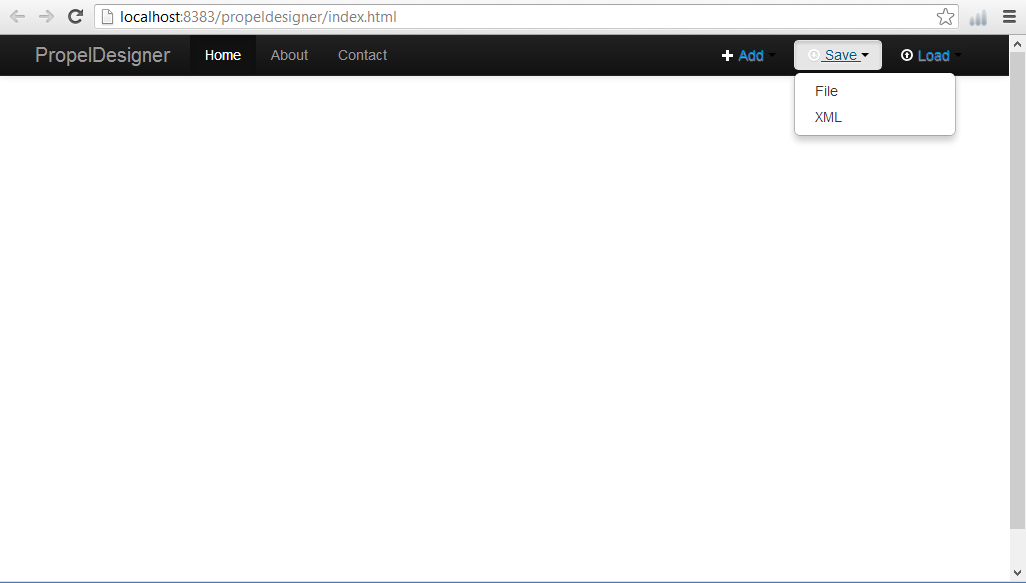
\includegraphics[width=15cm]{Images/blank_schema}
	\caption{This screen capture shows the SVG `canvas' in its initial, empty state. It also shows the UI features at the top of the screen and an example menu open.}
\end{figure}

\begin{figure}[h!]
	\centering
	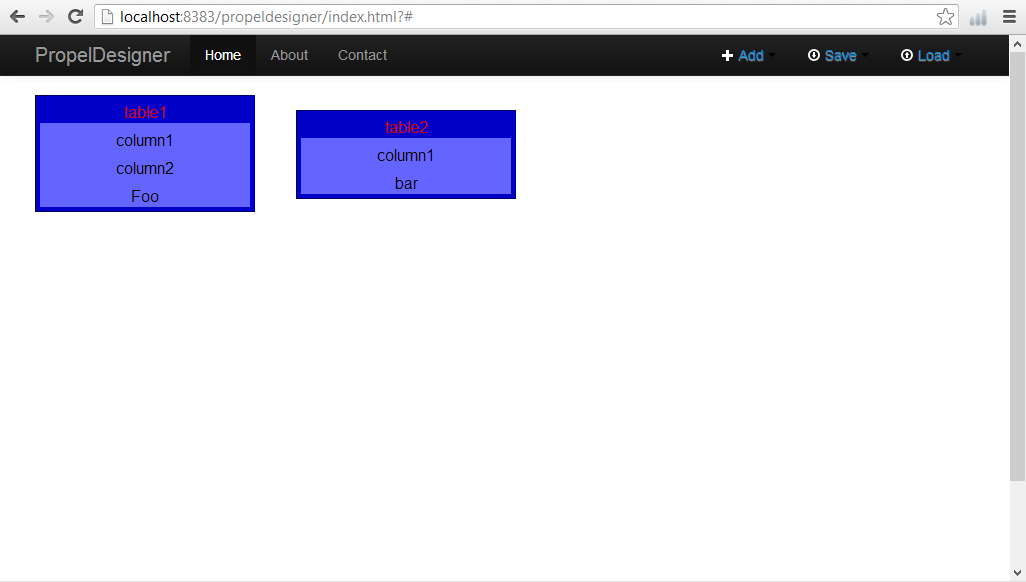
\includegraphics[width=15cm]{Images/populated_schema}
	\caption{This screen capture shows the SVG populated with two tables, each with a few columns. The colours are currently used to show to the developer the different parts of the SVG elements. The outermost rectangles (the tables) can be dragged around the SVG.}
\end{figure}

\begin{figure}[h!]
	\centering
	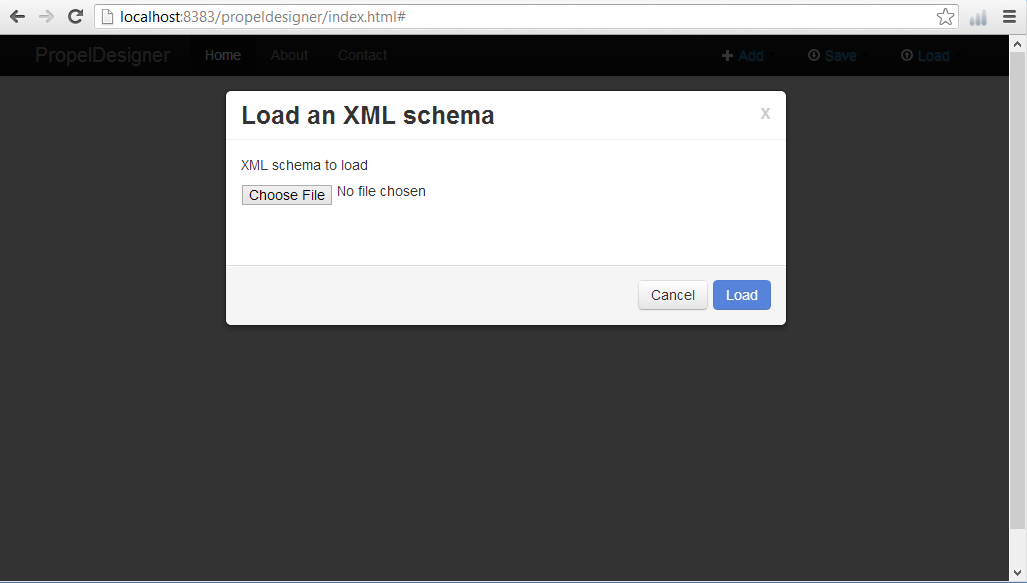
\includegraphics[width=15cm]{Images/open_file}
	\caption{This screen capture demonstrates the dialogue modal interface which, in this case, is showing the file load dialogue. The load button is disabled, here, as there is nothing to load.}
\end{figure}



\begin{figure}[h!]
	\centering
	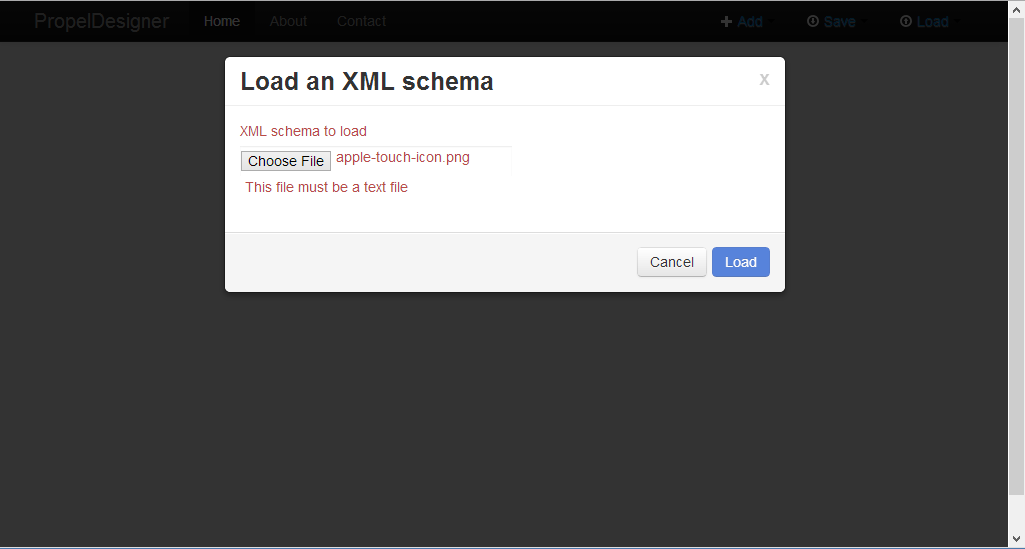
\includegraphics[width=15cm]{Images/open_error}
	\caption{This screen capture shows the previous screen capture, but where an incompatible file has been selected. This occurs without needing to load the file, using the File API in HTML5. The load button is still disabled. It will only become active when the file is of the text MIME type.}
\end{figure}

\fancypagestyle{plain}{%
   \fancyhead{} %[C]{Annotated Bibliography}
   \fancyfoot[C]{{\thepage} of \pageref{LastPage}} % except the center
   \renewcommand{\headrulewidth}{0pt}
   \renewcommand{\footrulewidth}{0pt}
}

\setemptyheader

\nocite{*} % include everything from the bibliography, irrespective of whether it has been referenced.

% the following line is included so that the bibliography is also shown in the table of contents. There is the possibility that this is added to the previous page for the bibliography. To address this, a newline is added so that it appears on the first page for the bibliography. 
\addcontentsline{toc}{chapter}{Annotated Bibliography} % Adds References to contents page

%
% example of including an annotated bibliography. The current style is an author date one. If you want to change, comment out the line and uncomment the subsequent line. You should also modify the packages included at the top (see the notes earlier in the file) and then trash your aux files and re-run. 
\bibliographystyle{authordate2annot}
%\bibliographystyle{IEEEannot}
\renewcommand{\bibname}{Annotated Bibliography} 
\bibliography{References/references} % References file


\end{document}
